\chapter{超荷、閉合與超空間}

\lectureoverview{超對稱之所以困難，不在於規則繁多，而在於這些規則把普通物理學中分開處理的觀念結合在一起。我們從格拉斯曼變數談起：它們的奇元素彼此反交換，而以這些變數為自變數的函數只會有有限項。格拉斯曼變數的微分代數，接著提供了奇對稱生成元的模型。玻色振子與費米振子構成最簡單的超荷：這些超荷的反對易子就是哈密頓量，因此玻色子與費米子的互換，和時間平移密不可分。同一代數也能以幾何方式表示：在稱為超空間的擴展時空中，沿格拉斯曼方向平移。}

\section{為什麼前進之前必須先退一步}

超對稱是物理學中最抽象的構造之一。它和旋轉、平移一樣是一種對稱性，但若不擴展座標的概念，就無法將它納入普通時空。它的自然參數是格拉斯曼量：這些物件可以相加、相乘，卻是反交換而非交換。

因此，直接處理最後的代數並不恰當。我們會先讓奇數的運算變得容易使用，再回顧普通連續對稱性如何組織，最後才把兩種觀念結合起來。這條路雖然較長，但每一步都為下一步鋪路。

\section{實用形式的格拉斯曼代數}

\subsection{奇元素與偶元素}

令 \(\epsilon_i\) 表示彼此獨立的格拉斯曼生成元。它們滿足
\begin{equation}
\epsilon_i\epsilon_j=-\epsilon_j\epsilon_i,
\qquad
\{\epsilon_i,\epsilon_j\}=0.
\end{equation}
令 \(i=j\)，便得到
\begin{equation}
2\epsilon_i^2=0,
\qquad
\epsilon_i^2=0,
\end{equation}
這些關係在實數或複數上成立。生成元本身不為零；為零的只有它的平方。

每個齊次元素都有奇偶性。含有奇數個格拉斯曼生成元的乘積是奇的，含有偶數個的乘積則是偶的：
\begin{align}
\text{odd}\times\text{odd}&=\text{even},\\
\text{odd}\times\text{even}&=\text{odd},\\
\text{even}\times\text{even}&=\text{even}.
\end{align}
偶元素與齊次元素交換，兩個奇元素則反交換。因此，當 \(n\) 為偶時，
\begin{equation}
n\epsilon_i=\epsilon_i n,
\qquad
\epsilon_i\epsilon_j=-\epsilon_j\epsilon_i,
\end{equation}

偶元素不一定是普通的實數或複數。例如，乘積 \(\epsilon_1\epsilon_2\) 是偶元素且為冪零。普通數構成代數中的純量部分；偶元素的乘積則提供其他可交換的元素。

\begin{classroomqa}
\audiencequestion{格拉斯曼代數和格拉斯曼數有區別嗎？還是兩者指的是同一回事？\lecturetimestamp{00:06:45}}
\lecturerresponse{格拉斯曼數是代數中的元素；格拉斯曼代數則是由這些元素，以及它們的加法和乘法規則所構成。因此，寬鬆地說兩者指的是同一個對象也可以，但區分運算的對象與運算規則仍有助於理解。}
\end{classroomqa}

\subsection{函數的展開會終止}

單一格拉斯曼變數的函數只有兩種可能的冪次：
\begin{equation}
f(\epsilon)=a+b\epsilon.
\end{equation}
不會有 \(\epsilon^2\) 項。若有兩個彼此獨立的生成元，
\begin{equation}
f(\epsilon_1,\epsilon_2)
=a+b_1\epsilon_1+b_2\epsilon_2+c\epsilon_1\epsilon_2.
\end{equation}
展開在兩個生成元都出現後便會終止。對於 \(n\) 個彼此獨立的生成元，有序單項式構成一組 \(2^n\) 維基底：
\begin{equation}
1,\quad
\epsilon_i,\quad
\epsilon_i\epsilon_j,\quad
\ldots,\quad
\epsilon_1\epsilon_2\cdots\epsilon_n.
\end{equation}
\editorialnote{有限的 \(2^n\) 維情形，概括了單一與兩個生成元的例子。也可以定義含有無限多個生成元的格拉斯曼代數，但這裡使用的多項式都只涉及有限個生成元。}

將兩個實生成元組成複數對 \(\theta,\bar\theta\) 後，一般函數可依選定的順序寫成
\begin{equation}
f(\theta,\bar\theta)
=a+\bar b\,\theta+\bar\theta\,b+c\,\bar\theta\theta.
\end{equation}
上方的橫線表示此處採用的複數對記號。若將最後兩個因子的順序顛倒，符號就會改變：
\begin{equation}
\bar\theta\theta=-\theta\bar\theta.
\end{equation}

通常，我們會為整個函數指定確定的奇偶性。若 \(f\) 為偶，則 \(a\) 和 \(c\) 為偶，\(b\) 和 \(\bar b\) 為奇。若 \(f\) 為奇，奇偶性便全部對調。係數本身可以屬於更大的格拉斯曼代數，只要它們不依賴於展開所用的那些特定變數。

\begin{classroomqa}
\audiencequestion{格拉斯曼變數可以代入三角函數或其他解析函數嗎？\lecturetimestamp{00:11:06}}
\lecturerresponse{可以，但冪級數很快就會終止。對單一奇生成元而言，
\[
\sin\epsilon=\epsilon,\qquad
\cos\epsilon=1,\qquad
e^\epsilon=1+\epsilon.
\]
函數仍沿用熟悉的名稱，但可用的冪次太少，無法呈現一般解析函數的複雜性。}
\end{classroomqa}

\section{微分就是符號的整理}

我們採用左格拉斯曼導數。它的局部定義規則為
\begin{equation}
\partial_\theta a=0,
\qquad
\partial_\theta(\theta B)=B,
\end{equation}
只要 \(a\) 和 \(B\) 不依賴 \(\theta\)，上述關係就成立。微分前，先將相關的 \(\theta\) 移到左側。每當它越過另一個奇因子，符號就會改變。

例如，若 \(b\) 為奇，
\begin{equation}
b\theta=-\theta b,
\qquad
\partial_\theta(b\theta)=-b.
\end{equation}
導數本身沒有任何神祕之處。負號是在微分之前、重新排列奇因子時產生的。

\subsection{雙變數的計算}

回到
\begin{equation}
f(\theta,\bar\theta)
=a+\bar b\,\theta+\bar\theta\,b+c\,\bar\theta\theta.
\end{equation}
先假設 \(f\) 為偶。於是 \(\bar b\) 為奇，\(c\) 為偶。重新排列含有 \(\theta\) 的項：
\begin{align}
\bar b\,\theta&=-\theta\bar b,\\
c\,\bar\theta\theta&=-\theta c\,\bar\theta.
\end{align}
因此
\begin{equation}
\partial_\theta f=-\bar b-c\bar\theta.
\end{equation}

若 \(f\) 為奇，則 \(\bar b\) 為偶，\(c\) 為奇。第一項不必越過任何奇係數；最後一項中的 \(\theta\) 則會越過兩個奇因子：\(c\) 和 \(\bar\theta\)。兩個負號彼此抵消：
\begin{equation}
\partial_\theta f=\bar b+c\bar\theta.
\end{equation}

\begin{classroomqa}
\audiencequestion{為什麼偶函數的例子中，留下的兩項都帶有負號？\lecturetimestamp{00:16:49}}
\lecturerresponse{第一個負號來自 \(\theta\) 越過奇係數 \(\bar b\)。在最後一項中，\(c\) 是偶的，但 \(\theta\) 必須越過奇變數 \(\bar\theta\)。每次重新排列都越過一個奇因子，因此各產生一個負號。}
\end{classroomqa}

答案取決於排列的約定，但數學本身不受影響。若一開始寫成 \(c\theta\bar\theta\) 而非 \(c\bar\theta\theta\)，顯示的係數就會差一個負號，導數公式也會相應改變。

\begin{classroomqa}
\audiencequestion{最後一項能否改寫成 \(\theta\) 和 \(\bar\theta\) 順序相反的形式？這樣產生的符號有更深層的意義嗎？\lecturetimestamp{00:18:50}}
\lecturerresponse{可以採用任一種順序，但交換兩個奇變數會改變符號。這個負號可以併入係數 \(c\)。在目前這個階段，這只是整理符號的問題：順序會影響正負號，奇偶性則不會改變；符號改變也絕不會把奇物件變成偶物件。當同樣的符號規則用來確保費米子統計和超對稱成立時，它才顯出物理意義。}
\end{classroomqa}

\begin{classroomqa}
\audiencequestion{係數 \(a,b,c\) 就只是取自複數域嗎？\lecturetimestamp{00:20:47}}
\lecturerresponse{若所需奇偶性為偶，係數可以是普通複數；也可以含有選定的 \(\theta,\bar\theta\) 以外的生成元。通常，所考慮的代數包含所有複數純量，以及一組選定的奇生成元與它們的乘積。}
\end{classroomqa}

\begin{classroomqa}
\audiencequestion{偶函數與奇函數的導數看起來互為相反數。這是一般性的對稱關係嗎？\lecturetimestamp{00:22:31}}
\lecturerresponse{不一定。符號是依照各係數的奇偶性，以及運算時越過了多少個奇因子逐步決定的。有時兩個結果恰好互為相反數，但可靠的規則更簡單：每交換兩個奇物件，就會多出一個負號。}
\end{classroomqa}

\subsection{座標與導數作為算符}

有一個很有啟發性的普通情形可供類比。令乘以 \(x\) 和對 \(x\) 微分這兩個運算作用於任意函數 \(g(x)\)，則
\begin{align}
\partial_x\!\left(xg\right)&=g+xg',\\
x\partial_xg&=xg',
\end{align}
所以
\begin{equation}
[\partial_x,x]g=g.
\end{equation}
由於這對任意 \(g\) 都成立，
\begin{equation}
[\partial_x,x]=1.
\end{equation}
取 \(p=-i\partial_x\)，便得到熟悉的位置與動量代數；這裡採用 \(\hbar=1\) 的單位制。

格拉斯曼變數的類比關係使用反對易子。令
\begin{equation}
f(\theta)=a+\theta b,
\end{equation}
其中 \(a\) 為偶、\(b\) 為奇，因此 \(f\) 為偶。先看
\begin{equation}
\theta\partial_\theta f=\theta b.
\end{equation}
再看相反的運算順序：
\begin{align}
\partial_\theta(\theta f)
&=\partial_\theta(\theta a+\theta^2b)\\
&=a.
\end{align}
將兩種順序的結果相加，便得到原函數：
\begin{equation}
\left(\partial_\theta\theta+\theta\partial_\theta\right)f
=a+\theta b=f.
\end{equation}
因此
\begin{equation}
\boxed{\{\partial_\theta,\theta\}=1.}
\end{equation}
導數 \(\partial_\theta\) 本身是奇的。這就是它與奇座標之間的正則關係採用反對易子的原因。

\begin{classroomqa}
\audiencequestion{可以使用同時含有偶部分和奇部分的函數，而不指定確定的奇偶性嗎？\lecturetimestamp{00:31:05}}
\lecturerresponse{這類非齊次元素可以構造出來，但計算通常會分別以齊次的偶物件和奇物件進行。指定確定的奇偶性，能讓分次乘積中的符號一目了然；混合物件則拆成偶部分與奇部分來處理。}
\end{classroomqa}

\begin{classroomqa}
\audiencequestion{在普通對易子的計算中，測試函數 \(g(x)\) 必須是奇函數嗎？\lecturetimestamp{00:31:45}}
\lecturerresponse{不必。它是普通可交換座標的普通函數。引入它只是為了說明算符恆等式 \([\partial_x,x]=1\) 如何證明，接著再以格拉斯曼變數對 \(\partial_\theta,\theta\) 重複同樣的論證。}
\end{classroomqa}

\begin{classroomqa}
\audiencequestion{獨立格拉斯曼生成元的數目有限制嗎？\lecturetimestamp{00:32:16}}
\lecturerresponse{代數上沒有上限。對 \(n\) 個生成元而言，基底有 \(2^n\) 個單項式，因此整理符號的工作會迅速增加，但此構造適用於任何有限的 \(n\)。}
\end{classroomqa}

\subsection{積分}

單一格拉斯曼變數的積分定義為
\begin{equation}
\int d\theta\,1=0,
\qquad
\int d\theta\,\theta=1.
\end{equation}
因此，對於 \(f(\theta)=a+\theta b\)，
\begin{equation}
\int d\theta\,f(\theta)=b=\partial_\theta f(\theta).
\end{equation}
積分與微分會提取相同的分量。這稱為貝雷津積分。這種歸一化方式是最簡單、且與平移不變性及格拉斯曼分部積分相容的選擇。\editorialnote{這些分量規則精確表達了講義中「格拉斯曼積分與微分是同一種運算」的說法。}

\section{以普通對稱性為基準}

考慮一個連續么正群，其厄米生成元為 \(G_i\)。在單位元附近，
\begin{equation}
U(\alpha)=\mathbf 1+i\alpha^iG_i+O(\alpha^2),
\end{equation}
其中 \(\alpha^i\) 是普通的可交換參數。無窮小乘法的規則由李代數描述：
\begin{equation}
[G_i,G_j]=i f_{ij}{}^{k}G_k.
\end{equation}
常數 \(f_{ij}{}^k\) 稱為結構常數。所謂閉合，是指任意兩個生成元的對易子都會回到代數中，成為既有生成元的線性組合。

對於轉動，
\begin{equation}
[L_i,L_j]=i\varepsilon_{ijk}L_k.
\end{equation}
三個厄米分量可組合成非厄米的升降算符：
\begin{equation}
L_\pm=L_x\pm iL_y,
\end{equation}
它們會使磁量子數 \(m\) 增加或減少一。複數線性組合雖然方便，但不會改變底層物理生成元的厄米性。

在一般基底下，\(f_{ij}{}^k\) 只有前兩個指標必須反對稱。對於具有不變正交度量的緊緻李代數，可以降低最後一個指標，並選擇適當的約定，使 \(f_{ijk}\) 完全反對稱，就如同轉動代數的情形。\editorialnote{這個限定說明，對易子的反對稱性普遍成立；熟悉的轉動基底還具有更強的性質。}

若要讓 \(G_i\) 成為時間無關系統的對稱性生成元，就必須有
\begin{equation}
[H,G_i]=0.
\end{equation}
等價地說，\(G_i\) 會將每個能量本徵空間映射到自身。若系統沒有顯式的時間依賴，海森堡方程給出
\begin{equation}
\frac{dG_i}{dt}=i[H,G_i]=0,
\end{equation}
因此這個生成元是守恆荷。

普通可觀測量是偶的。費米子場是奇的，但單獨的奇場本身不是可測量的可觀測量；物理算符中的費米子因子總數必須是偶數。超對稱改變的是生成元的奇偶性，不是可觀測結果所要求的奇偶性。

適用於各種情形的簡潔記號是分次對易子：
\begin{equation}
[X,Y]_{\mathrm{gr}}
=XY-(-1)^{|X||Y|}YX.
\end{equation}
若兩個算符中至少有一個是偶的，它就是普通對易子；若兩者都是奇的，它就是反對易子。

\section{最簡單的超對稱振子}

\subsection{一個玻色模與一個費米模}

考慮單一玻色模，其產生算符與湮滅算符分別為 \(a_+\) 和 \(a_-\)：
\begin{equation}
[a_-,a_+]=1,
\qquad
[a_+,a_+]=[a_-,a_-]=0.
\end{equation}
其數算符為
\begin{equation}
N_B=a_+a_-,
\end{equation}
佔據數可以是 \(0,1,2,\ldots\)。

對單一費米模，引入 \(c_+\) 和 \(c_-\)：
\begin{equation}
\{c_-,c_+\}=1,
\qquad
\{c_+,c_+\}=\{c_-,c_-\}=0.
\end{equation}
因此
\begin{equation}
c_+^2=c_-^2=0,
\qquad
N_F=c_+c_-,
\end{equation}
佔據數只能是 \(0\) 或 \(1\)。玻色算符為偶，費米算符為奇，而且任一 \(a_\pm\) 都與任一 \(c_\pm\) 對易。

\editorialnote{冪零性將費米模限制為最多一個粒子佔據。玻色模的佔據數則不受限制；課堂討論中一處簡短的相反說法，可由振子代數本身釐清。}

假設玻色子與費米子具有相同的靜止能量 \(m\)，並定義
\begin{equation}
Q=\sqrt m\,a_+c_-,
\qquad
\bar Q=Q^\dagger=\sqrt m\,a_-c_+.
\end{equation}
算符 \(Q\) 會移除一個費米子並產生一個玻色子；它的共軛算符則移除一個玻色子並產生一個費米子。兩者都含有一個費米算符，因此都是奇的。

在數態上的作用如下：
\begin{align}
Q\ket{n,1}
&=\sqrt{m(n+1)}\,\ket{n+1,0},
&
Q\ket{n,0}&=0,\\
\bar Q\ket{n,0}
&=\sqrt{mn}\,\ket{n-1,1},
&
\bar Q\ket{n,1}&=0.
\end{align}
\editorialnote{這些數態公式直接給出講義所述粒子替換作用的歸一化形式。}

\subsection{反對易子閉合為能量}

尋找李代數的分次類比，可從計算下式開始：
\begin{align}
\{Q,\bar Q\}
&=Q\bar Q+\bar Q Q\\
&=m\left(a_+c_-a_-c_+
        +a_-c_+a_+c_-\right).
\end{align}
由於 \(a\) 是偶的，它們通過 \(c\) 時不會產生負號：
\begin{equation}
\{Q,\bar Q\}
=m\left(a_+a_-c_-c_+
        +a_-a_+c_+c_-\right).
\end{equation}
接著使用
\begin{equation}
c_-c_+=1-c_+c_-,
\qquad
a_-a_+=a_+a_-+1.
\end{equation}
可得
\begin{align}
\{Q,\bar Q\}
&=m\left[
N_B(1-N_F)+(N_B+1)N_F
\right]\\
&=m(N_B+N_F).
\end{align}
逐步重排時一度出現的額外因子 2，最後會消去：一項給出 \(N_B\)，另一項給出 \(N_F\)。

對於靜止且質量相同的粒子，哈密頓量為
\begin{equation}
H=m(N_B+N_F).
\end{equation}
因此
\begin{equation}
\boxed{\{Q,\bar Q\}=H.}
\end{equation}

\begin{figure}[H]
\centering
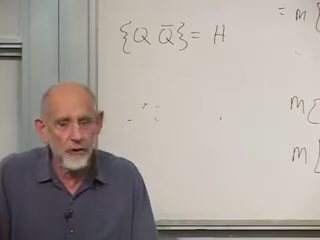
\includegraphics[width=0.62\textwidth]{lecture_05_figure_02.png}
\lectureframe{00:55:46.300}
\caption{黑板上單獨寫出的核心閉合關係。圖中可見花括號和 \(Q,\bar Q,H\)；逗號則依標準反對易子記法補出。}
\end{figure}

能量的加法零點選定為使真空態滿足 \(H=0\)。對超對稱振子而言，這是自然的約定：玻色與費米的零點能貢獻會互相抵消。\editorialnote{講義直接使用總靜止能量，沒有分別列出零點能項；這項約定明確說明了所採用的選擇。}

哈密頓量是偶的，也是一個對稱性生成元：它生成時間平移。因此，若不將偶的時間平移生成元納入，奇生成元就無法彼此閉合。

\begin{classroomqa}
\audiencequestion{這個關係式中哪一項是偶的？是哈密頓量嗎？\lecturetimestamp{00:58:24}}
\lecturerresponse{是。能量是普通的可觀測量，所以 \(H\) 是偶的。超荷 \(Q\) 是奇的，而兩個奇量的乘積是偶的，因此 \(\{Q,\bar Q\}\) 可以等於 \(H\)。奇生成元與偶生成元之間的關係由對易子表示，而不是反對易子。}
\end{classroomqa}

\subsection{補全代數}

同奇偶性的關係式很直接：
\begin{equation}
\{Q,Q\}=2Q^2=0,
\qquad
\{\bar Q,\bar Q\}=2\bar Q^2=0,
\end{equation}
因為 \(Q^2\) 含有 \(c_-^2\)，而 \(\bar Q^2\) 含有 \(c_+^2\)。

接下來要找出它與 \(H\) 的關係。令
\begin{equation}
H\ket{E}=E\ket{E}.
\end{equation}
若玻色子與費米子的質量相等，\(Q\) 會將其中一者轉換為另一者，而不改變能量。因此，\(Q\ket{E}\) 不是零，就是另一個具有相同本徵值的本徵態：
\begin{equation}
H Q\ket{E}=E Q\ket{E}.
\end{equation}
另一方面，
\begin{equation}
QH\ket{E}=Q(E\ket{E})=E Q\ket{E}.
\end{equation}
兩式相減，得到
\begin{equation}
[H,Q]\ket{E}=0.
\end{equation}
若能量本徵態構成完備基底，便可將此結果提升為算符恆等式：
\begin{equation}
[H,Q]=0,
\qquad
[H,\bar Q]=0.
\end{equation}

\begin{classroomqa}
\audiencequestion{如果玻色子與費米子的質量不相同，會發生什麼事？\lecturetimestamp{01:01:16}}
\lecturerresponse{這時將一者轉換成另一者會改變能量，因此所定義的超荷不會與哈密頓量對易，簡單的超對稱性便不成立。對於
\[
H=m_BN_B+m_FN_F,
\]
直接計算可得
\[
[H,Q]=(m_B-m_F)Q.
\]
此式恰在 \(m_B=m_F\) 時為零。\editorialnote{不等質量時的對易子，直接以算符形式表達了能量改變的論證，也明確顯示質量相等的條件。}}
\end{classroomqa}

\begin{classroomqa}
\audiencequestion{能不能更仔細地說明能量本徵態的論證？\lecturetimestamp{01:01:37}}
\lecturerresponse{先從 \(H\ket{E}=E\ket{E}\) 開始。質量相等表示 \(Q\ket{E}\) 具有確定能量 \(E\)，所以 \(HQ\ket{E}=EQ\ket{E}\)。改變運算順序則得到 \(QH\ket{E}=QE\ket{E}=EQ\ket{E}\)，因為 \(E\) 是普通純量。兩者相減後，在每個能量本徵態上都為零。利用本徵態的完備性，就能將這個結論提升為算符方程 \([H,Q]=0\)。}
\end{classroomqa}

因此，完整的玩具模型代數為
\begin{align}
\{Q,\bar Q\}&=H,\\
\{Q,Q\}&=\{\bar Q,\bar Q\}=0,\\
[H,Q]&=[H,\bar Q]=0.
\end{align}
超荷是守恆的奇荷。更令人驚訝的是，它們的代數把改變粒子種類的運算，與時空平移的生成元連結起來。

\section{哈密頓量為何代表時間平移}

這個簡化模型沒有空間座標，但有時間。薛丁格方程為
\begin{equation}
i\frac{\partial}{\partial t}\ket{\psi(t)}
=H\ket{\psi(t)}.
\end{equation}

\begin{figure}[H]
\centering
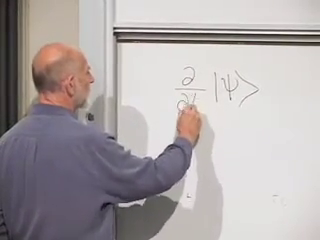
\includegraphics[width=0.56\textwidth]{lecture_05_figure_03.png}
\lectureframe{01:07:26.300}
\caption{時間導數寫在 \(\ket{\psi}\) 旁邊。手遮住了分母的一部分；完整的薛丁格方程已列於上方。}
\end{figure}

對於有限的時間位移 \(\delta\)，
\begin{equation}
\ket{\psi(t+\delta)}
=e^{-iH\delta}\ket{\psi(t)}.
\end{equation}
展開至一階，得
\begin{equation}
\ket{\psi(t+\delta)}
=\left(\mathbf 1-i\delta H\right)\ket{\psi(t)}
+O(\delta^2).
\end{equation}
因此，\(H\) 是使態隨時間演化的無窮小生成元。

同位旋和色等內部對稱性也會改變粒子標記。同位旋可以混合質子態與中子態；色旋轉則混合紅、綠、藍夸克。然而，這些內部變換無論如何組合，都不會使系統在空間或時間中平移。超對稱則不同：
\begin{equation}
\begin{gathered}
\text{odd particle-changing transformation}\\
\mathrel{\stackrel{\{\ ,\ \}}{\Longrightarrow}}\\
\text{time translation}
\end{gathered}
\end{equation}
這提示我們，奇生成元本身可能就是平移，只是平移方向不同於通常的方向。

\section{超空間}

\subsection{時間與奇座標的函數}

引入函數
\begin{equation}
\Psi=\Psi(\theta,\bar\theta,t).
\end{equation}
在玩具模型中，它可以視為波函數；更一般地說，則可視為超場。由於對奇變數的展開會終止，
\begin{equation}
\Psi(\theta,\bar\theta,t)
=A(t)+\bar\chi(t)\theta
+\bar\theta\chi(t)+F(t)\bar\theta\theta.
\end{equation}
單一物件便包含了偶分量函數與奇分量函數。\editorialnote{這個分量展開運用了前面介紹的格拉斯曼多項式，明確呈現了玩具超空間上函數的標準形式。}

普通的時間平移會使 \(\theta,\bar\theta\) 保持不變，並令
\begin{equation}
t\longmapsto t+\delta.
\end{equation}
展開至一階，得
\begin{equation}
\Psi(\theta,\bar\theta,t+\delta)
=\Psi(\theta,\bar\theta,t)
+\delta\,\partial_t\Psi(\theta,\bar\theta,t).
\end{equation}

\begin{figure}[H]
\centering
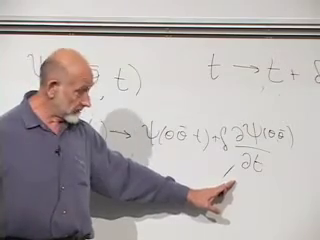
\includegraphics[width=0.72\textwidth]{lecture_05_figure_04.png}
\lectureframe{01:13:15.060}
\caption{黑板上在 \(t\to t+\delta\) 上方寫出 \(\Psi\) 的一階變化，並直接標示其導數項。}
\end{figure}

\subsection{沿奇方向平移}

現在定義一個平移奇座標的變換：
\begin{equation}
\theta\longmapsto\theta+\epsilon,
\end{equation}
其中 \(\epsilon\) 是另一個奇的格拉斯曼參數。同時，讓時間產生一個偶的冪零位移：
\begin{equation}
t\longmapsto t+i\bar\theta\epsilon.
\end{equation}
\(\bar\theta\) 和 \(\epsilon\) 都是奇的，因此兩者的乘積為偶，可以一致地加到偶座標 \(t\) 上。

將參數移到左側後，
\begin{equation}
i\bar\theta\epsilon=-i\epsilon\bar\theta.
\end{equation}
因此誘發的變化為
\begin{align}
\delta_\epsilon\Psi
&=\epsilon\,\partial_\theta\Psi
-i\epsilon\bar\theta\,\partial_t\Psi\\
&=\epsilon q_0\Psi,
\end{align}
其中
\begin{equation}
q_0=\partial_\theta-i\bar\theta\partial_t.
\end{equation}
這個奇微分算符生成上述組合平移。使用左導數時，與之相容的共軛生成元為
\begin{equation}
\bar q_0=-\partial_{\bar\theta}
+i\theta\partial_t.
\end{equation}

具體的符號取決於使用左格拉斯曼導數或右格拉斯曼導數，以及共軛運算如何反轉奇因子的順序。無論採用哪種約定，代數都必須閉合於時間平移。依照上述定義，
\begin{align}
\{q_0,\bar q_0\}
&=i\{\partial_\theta,\theta\}\partial_t
+i\{\bar\theta,\partial_{\bar\theta}\}\partial_t\\
&=2i\partial_t.
\end{align}
導數與導數的乘積項會消失，奇座標的二次項也會消失。兩個混合項各自貢獻 \(i\partial_t\)。

由於薛丁格繪景中的態滿足 \(H=i\partial_t\)，
\begin{equation}
\{q_0,\bar q_0\}=2H.
\end{equation}
若作如下歸一化：
\begin{equation}
q=\frac{q_0}{\sqrt2},
\qquad
\bar q=\frac{\bar q_0}{\sqrt2},
\end{equation}
則
\begin{equation}
\boxed{\{q,\bar q\}=H.}
\end{equation}
\editorialnote{講義刻意逐步處理不確定的符號，最後注意到多出一個因子 2。這裡展示的左導數約定保留了課堂上的計算過程，同時採用一種自洽的歸一化。其他標準約定會將符號的差異分配到座標平移與生成元之中。}

\begin{classroomqa}
\audiencequestion{超空間反對易子最後的因子 2 從何而來？\lecturetimestamp{01:24:21}}
\lecturerresponse{這裡有兩個相等的混合項。一項來自 \(\{\partial_\theta,\theta\}=1\)，另一項來自 \(\{\partial_{\bar\theta},\bar\theta\}=1\)；兩者都乘上時間導數。因此，未歸一化的生成元給出 \(2i\partial_t\)；在每個超荷中乘上因子 \(1/\sqrt2\)，就能恢復先前採用的歸一化。}
\end{classroomqa}

\begin{classroomqa}
\audiencequestion{這個構造是否假設 \(\epsilon\) 很小？\lecturetimestamp{01:24:51}}
\lecturerresponse{這裡用到的是冪零性，而不是普通數值意義上的大小。由於 \(\epsilon^2=0\)，以單一 \(\epsilon\) 展開時，所有項都會在一階後終止。稱它為無窮小或很小，是有用的類比，但截斷是精確的。}
\end{classroomqa}

\editorialnote{格拉斯曼參數沒有普通數值所具有的正大小。它之所以扮演無窮小參數的角色，是因為它具有冪零性，且展開會精確終止。}

\subsection{幾何意義}

這個代數現在有兩種等價的實現方式。在振子圖像中，\(Q\) 和 \(\bar Q\) 會分別將費米子轉換為玻色子、將玻色子轉換為費米子。在幾何圖像中，\(q\) 和 \(\bar q\) 沿奇方向平移函數，同時誘發普通的時間平移。在這兩種圖像中，
\begin{equation}
\begin{gathered}
\{\text{supercharge},\text{conjugate supercharge}\}\\
=\text{time-translation generator}.
\end{gathered}
\end{equation}

包含 \(t,\theta,\bar\theta\) 的廣義座標空間稱為超空間。在相對論性場論中，超空間還包含普通空間座標，而超荷閉合於完整的時空動量 \(P_\mu\)，不只閉合於 \(H=P_0\)。將這種結構彎曲，便會走向超引力。

格拉斯曼變數一方面是有效整理玻色子與費米子計算的工具；另一方面，閉合關係也揭示了更深一層的意義：粒子種類與時空幾何之間的區分不再是絕對的。沿奇方向平移兩次，會產生沿普通方向的位移。自然界是否在實驗上實現了這種結構，是另一個問題；在數學上，這套結構自洽、簡潔，而且具有驚人的剛性。
